\section{Estimativa de corrente máxima}

% * 2024-05-13-SI_max_stored_current_estimate (maximum-beam-current-estimate)


\begin{frame}{Estimativa de corrente máxima}

{\footnotesize
\begin{itemize}
    % \setlength\itemsep{1em}
    \item estudo dia 2024-05-13 \href{https://cnpemcamp.sharepoint.com/:b:/s/FAC/EYc5lGyqOatKoH_Rp2DNA1oBWygwBlE_1N8TA8AZYdNcBw?e=wTYFhx}{\beamergotobutton{Teams FAC/Machine Studies/Files}}
    \item dois trens de pacotes centrados nos buckets 260 e 292, acumulando e acompanhando as temperaturas dos componentes do anel
    \item conseguimos chegar em 90 mA (equivalente a feixe uniforme de 220 mA) 
    \item sensor MD4 (bellows entre scraper vertical e dipolo) chegou a 49$^\circ$C
    \item top-up por 1h em 90 mA $\rightarrow$ 80 mA, mais tempo e MD4 foi para 47$^\circ$C
    \item 4 bellows do TR01 são elípticos, enquanto outros são circulares (estes não aqueceram).
    \item somente o MD4 aqueceu, outros 3 não: o MD4 deve ter alguma particularidade mecânica.
\end{itemize}
}
% \vspace{-0.3cm}
\begin{figure}[ht]
    \centering
    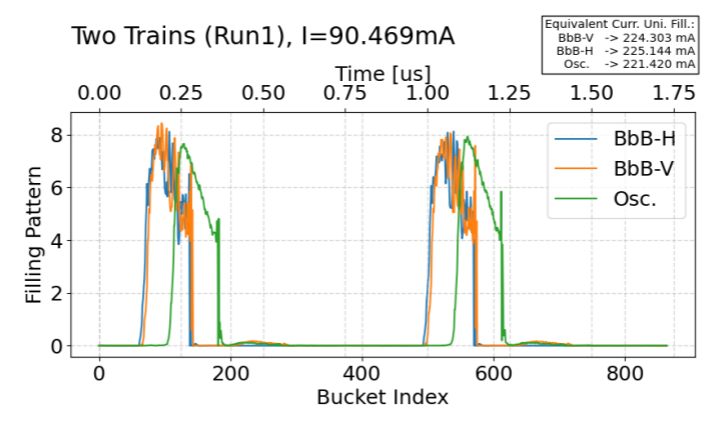
\includegraphics[height=3.2cm]{2024-07-12/figures/filling-pattern.png}
\end{figure}
\end{frame}